\documentclass{article}

% if you need to pass options to natbib, use, e.g.:
%     \PassOptionsToPackage{numbers, compress}{natbib}
% before loading neurips_2022

% ready for submission
\usepackage[preprint]{neurips_2022}

% to compile a preprint version, e.g., for submission to arXiv, add add the
% [preprint] option:
%     \usepackage[preprint]{neurips_2020}

% to compile a camera-ready version, add the [final] option, e.g.:
%     \usepackage[final]{neurips_2020}

% to avoid loading the natbib package, add option nonatbib:
%\usepackage[nonatbib]{neurips_2020}
\usepackage[utf8]{inputenc} % allow utf-8 input
\usepackage[T1]{fontenc}    % use 8-bit T1 fonts
\usepackage{hyperref}       % hyperlinks
\usepackage{url}            % simple URL typesetting
\usepackage{booktabs}       % professional-quality tables
\usepackage{amsfonts}       % blackboard math symbols
\usepackage{nicefrac}       % compact symbols for 1/2, etc.
\usepackage{microtype}      % microtypography


% Graphics and color
\usepackage{graphicx}
\usepackage{xcolor}

% References and Bibliography
\usepackage{url}
\usepackage{hyperref}
\hypersetup{
  colorlinks,
  linkcolor={black},
  citecolor={blue!50!black},
  urlcolor={blue!50!black}
}
\usepackage{cleveref}
\usepackage[numbered]{bookmark} % Fixes false PDF table of contents
\usepackage{natbib}
\setcitestyle{numbers,sort&compress,square,comma}
\usepackage{bibentry}
\nobibliography*

\title{Can Plant-based Diets Help Solve Climate Change?}


\author{%
  Hanna Dettki\thanks{Equal contribution.} \\
  Department of Computer Science\\
  University of Tübingen\\
  \texttt{hanna.dettki@student.uni-tuebingen.de} \\
  \And
  Davide $^{*}$  \\
  Department of Computer Science\\
  University of Tübingen\\
  \texttt{@student.uni-tuebingen.de} \\
  % \AND
  % Coauthor \\
  % Affiliation \\
  % Address \\
  % \texttt{email} \\
  % \And
  % Coauthor \\
  % Affiliation \\
  % Address \\
  % \texttt{email} \\
  % \And
  % Coauthor \\
  % Affiliation \\
  % Address \\
  % \texttt{email} \\
}

\begin{document}

\maketitle

\begin{abstract}
  This research is made for the Data Literacy Project of the academic year 2022/2023. It covers the discussion about the emissions of a plant based diet in comparison with a traditional diet. The research is conducted by exploration of the data, hypothesis testing and example comparisons. 
\end{abstract}

\section{Introduction}

Climate change threatens everyone. In order to avoid a climate disaster, radical change is needed. This concerns everything, from policies on a global and national level, to choices taken by the individual on a daily basis. 
However, individuals motivated and willing to solve climate change by pursueing a sustainable life are faced with many obstacles to do so effortlessly. Food, energy and water is what the UN refer to as the culprit for a sustainable world, whose population has expanded and whose demand has increased for all three of the aforementioned  \cite{Ritchie2020}.
 Importantly, food systems are responsible for a third of global anthropogenic greenhouse gas emissions \cite{Crippa2021}. At the same time, food choices are to a large extent up to the individuum.  Tragically,  the emission of food options are not handily accessible to the individuum, which is why one is not able to take an informed climate friendly food decision. This shows that a significant lever contributing to solving climate change is not pulled!
\paragraph*{Research Question}
Therefore, we investigate the environmental impact of the most common food categories, which is a first step towards  providing more information in the jungle of food choices that everybody is presented with. In particular, we hypothesize that  plant-based diets  have a significantly smaller CO$_2$-footprint than  diets including animal-derived products in the typical Western diet.

\section{Data}
\label{data}
\paragraph{Data generating process} \label{dataGen}
The data used in this analysis  is the largest meta-analysis of food systems to date and was published in the journal \textit{Science} by \citet{Poore2018}.
570 studies met the eleven criteria\footnote{Such as  methodologies used were standardized, e.g., that all stages of the supply chain were considered.} \citet{Poore2018}  were applying to the initially  1530 studies.
The final dataset covers approximately 38,700 farms across 119 countries and spans a total of 40 food products, which represent approximately 90\% of global protein and calorie intake. The breadth of this analysis ensures that results are only minimally biased towards any geographic region,  any particular faming method or income level.
\paragraph*{Greenhouse gases (GHG) and how they are quantified}
Since there are many different greenhouse gases (GHG), researchers commonly aggregate them into a measurement that is easy to use for comparisons. 
\citet{Poore2018} use the metric 
``carbon dioxide-equivalents (CO$_{2}$eq)'', which is the most common measurement and is for instance  also used as a target-setting metric in official reportings like the Paris Agreement. CO$_{2}$eq express the ``global warming potential'' by aggregating the impact of all GHG into a single metric  and  aims to represent the amount of warming that each specific gas generates relative to CO$_2$. The ``global warming potential over a $100$-year timescale (GWP$_{100}$)'' expresses the mid- to longterm period for climate-policies. To calculate the CO$_{2}$eq-value, the amount of each GHG needs to factorized by its GWP$_{100}$-value. For example, the Intergovernmental Panel on Climate Change (IPCC) sets the GWP$_{100}$-value of the GHG  methane to $28$, which is based on the rationale that methane's global warming impact over a period of 100 years, will be $28$ times higher than that of one kilogram of CO$_2$.
\paragraph{Stages of supply chain}
Note: only if included in analysis
% Land use change; 
% On-farm impacts in crop or livestock production (including the manufacturing of inputs such as fertilizers, or emissions from manure);
% Animal feed production;
% Food processing: the conversion of raw ingredients into sold products, such as the processing of cereals into bread;
% Transport: this includes transport from the farm up to retail. Transport of food from retail to consumers’ homes is not included.
% Packaging
% Retail: energy consumption in retail stores, such as refrigeration.



\paragraph{Dataset adaptions and handling of missing data}

We substituted  missing  data by taking the mean of the existing values of the respecting feature. To facilitate data queries, we added a column "Plant-based", which holds binary values $[0,1]$ and indicates whether a product is plant-based $(1)$ or animal-derived $(0)$.


\section{Analysis}
\label{analysis}

To get an overview as to which features of the dataset provide most information, we calculated the pairwise correlation of a subset of features. Given a pair of random variables $(X,Y)$, the population Pearson correlation coefficient is: 
\begin{equation} \label{eq:corr}
  \rho_{X,Y} = \frac{cov(X,Y)}{\sigma_X \sigma_Y}
\end{equation}
where $cov(X,Y)$ is the covariance, $\sigma_X$ is the standard deviation of $X$ and $\sigma_Y$ is the standard deviation of $Y$.
\Cref{eq:corr} applied to the features is depicted  as a heat-map in  \Cref{fig:corr}.  \Cref{fig:corr} illustrates that
plant-based products are strongly correlated ($|\rho| \in [1.00 - 0.5]$) with every other feature except for \textit{Transport} and \textit{Packaging}. This is indicative of our hypothesis that plant-based products emit significantly less than animal-derived products stated in  \Cref*{data}.


\begin{figure}[h]
  \centering
  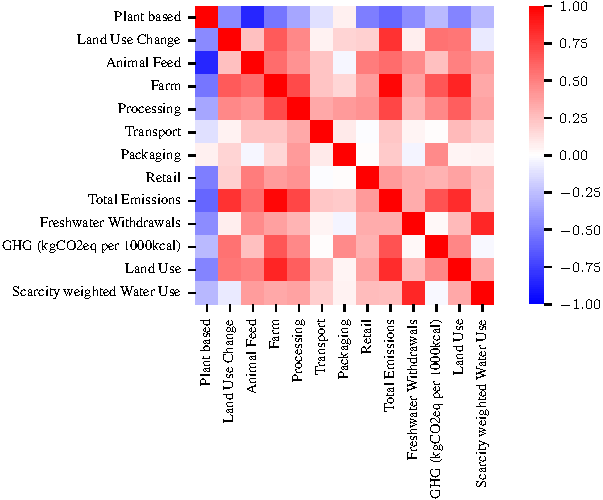
\includegraphics[width=0.65\textwidth]{figures/heat-map.pdf}
  \caption{Correlation of a subset of features depicted in a heat-map. Plant-based products are  correlated ($|\rho| \in [1.00, 0.5]$) with every other feature except for \textit{Transport} and \textit{Packaging}.}
  \label{fig:corr}
\end{figure}

\subsection*{Hypothesis Testing}
In order  to decide as to whether the data supports our hypothesis, we will run a T-test, which tests, if the two distributions have equal means (Null-hypothesis). W Since the samples are neither of same size, nor of same variance and are assumed to be independent, we opt for the independent unequal variance T-Test, also known as \textit{Welch's Test}. %\cite{WelchTest}. 
%\cite{WelchTest} 
The test-statistic is computed as follows:
\begin{equation}\label{eq:t-test}
  t = \frac{\bar{X}-\bar{Y}}{\sqrt{\sigma^2_{X}+\sigma^2_{Y}}}
\end{equation}
where $\bar{X}$ and  $\bar{Y}$ are the sample mean with respective standard deviation $\sigma_{X,Y}$.

\subsubsection*{Do plant- and non-plant-based food products significantly differ w.r.t. their total emissions?}


 We will consider \textit{plant-based} and \textit{not plant-based} w.r.t.  the two features \textit{Total emissions} and \textit{GHG} respectively.
\paragraph*{Kernel-density-estimation to check for distribution family} Since \textit{Welch's Test} assumes implicitly Gaussian-distributed data, we should first check the distribution family that  our data belongs to, in order to make sure that the selected test is appropriate. We therefore generate a histogram and estimate the kernel density with the Python package Seaborn. Plant-based and not-plant-based food categories are depicted w.r.t their total emissions in \Cref{fig:emissions}.
\begin{figure}[h]\label{fig:emissions}
  \centering
  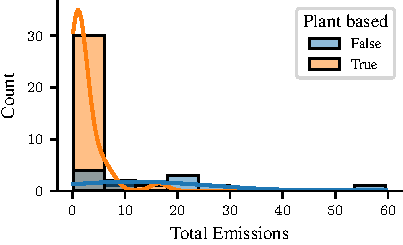
\includegraphics[width=0.65\textwidth]{figures/emissions.pdf}
  \label{fig:emissions}
\end{figure}
Analyzing \Cref{fig:emissions}, two things can be concluded: First, our hypothesis, that the plant-based and animal-based food products have two different underlying distributions can be confirmed. Second, the distribution over total emissions of plant-based products clearly does not follow a Gaussian distribution. 

\paragraph*{Data-transformation}
In order to transform the data to Gaussian-like distributions, we apply the logarithm with basis $10$ to the data. We can do this, since the logarithm is a monotonic function and will hence not shift the location of the mean. Applying the logarithm, we obtain the kernel density estimation depicted in \Cref{fig:emissions-log} 

\begin{figure}[h]
  \centering
  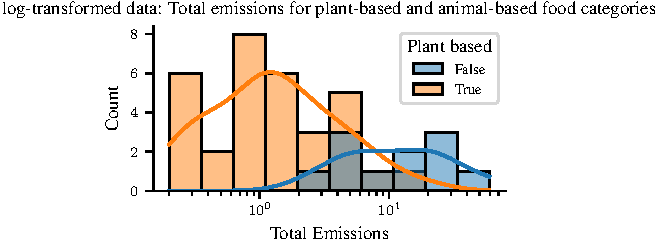
\includegraphics[width=0.65\textwidth]{figures/emissions-log.pdf}
  \label{fig:emissions-log}
\end{figure}


\subsubsection*{Accounting  for Nutritional Value: Do plant- and non-plant-based food products significantly differ w.r.t. their GHG?}


Now, we will consider \textit{plant-based} and \textit{not plant-based} w.r.t.  the feature \textit{GHG}.



\begin{figure}[h]
  \centering
  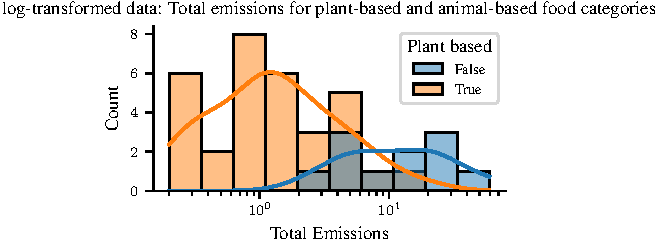
\includegraphics[width=0.65\textwidth]{figures/emissions-log.pdf}
  \label{fig:emissions-log}
\end{figure}

\begin{figure}[h]
    \centering
    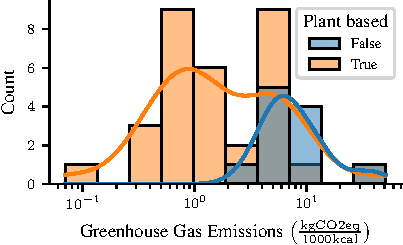
\includegraphics{figures/ghg-log.pdf}
    \label{fig:ghg-log}
\end{figure}



\subsection{Comparing Typical Diets}
\section{Results}
\begin{table} \label{tbl:results}
  \caption{Results of applying Welch's Hypothesis Test}
  \label{sample-table}
  \centering
  \begin{tabular}{lll}
    \toprule
    %\multicolumn{1}{c}{}&\multicolumn{2}{c}{Plant-based} &%\multicolumn{2}{c}{Animal-based}                   \\
    %\cmidrule(r){2-5}
    Feature     & Test-Statistic   & p-value  \\
    \midrule
    Total Emissions &$\sim$6.49  & $\sim$0.00022\%    \\
    GHG     & $\sim$5.03   & $\sim$0.0014\%   \\
    \bottomrule
  \end{tabular}
\end{table}

\section{Conclusion}
\label{conclusion}


\section{Limitations and Outlook}
\label{limitations}
How methane is treated which is a shorter-lived, but more powerful greenhouse gas than CO2  is often discussed.

Unfortunately data is not available to present this breakdown by country or region

Compare difference between the worst and best producers. This means there is an opportunity to reduce the impacts of food production by optimizing for the lowest-impact producers. However, what is also clear is that this does not change the ordering of the impacts of different foods. It's still the case that nearly all beef and lamb producers have a high carbon footprint higher than plant-based alternatives, even if we opt for the best(lowest-impact) producers.
\begin{itemize}
  \item reducing GHG
  \item animal welfare
  \item biodiversity
  \item Health: While there are some concerns, that vegan diets (i.e, plant-based diets that exclude all forms of animal products in their entirety) are not sufficient w.r.t providing recommended micronutiernt levels (e.g. vitamin B12, zinc, iron, etc.), they generally meet protein intake recommendations. Nonetheless, individuals who consume a vegan diet should remain aware regarding potential micronutirent insufficiencies. 
  \end{itemize}
  
{\small
\bibliographystyle{unsrtnat}
\bibliography{../literature/references.bib}
}
\end{document}
